

\documentclass	{xmgr}
\usepackage{listings}
% Jeśli nowe rozdziały mają się zaczynać na stronach
% nieparzystych:
%\documentclass[openright]{xmgr}

%\defaultfontfeatures{Scale=MatchLowercase}
%\setmainfont[Numbers=OldStyle,Ligatures=TeX]{Minion Pro}
%\setsansfont[Numbers=OldStyle,Ligatures=TeX]{Myriad Pro}
% for fontspec version < 2.0
%\setmonofont[Scale=0.75]{Monaco}
\setmainfont[Numbers=OldStyle,Mapping=tex-text]{Minion Pro}
\setsansfont[Numbers=OldStyle,Mapping=tex-text]{Myriad Pro}

% Opcjonalnie identyfikator dokumentu
% drukowany tylko z włączoną opcją 'brudnopis':
\wersja   {wersja wstępna [\ymdtoday]}

\author   {Adrian Pieper}
\nralbumu {243\,677}
\email    {adrpieper@gmail.com.pl}

\title    {Adventure Maker...}
\date     {2017}
\miejsce  {Gdańsk}

\opiekun  {dr W. Bzyl}

% dodatkowe polecenia
%\renewcommand{\filename}[1]{\texttt{#1}}
%\definecolor{stress}{cmyk}{0,1,0.13,0} % RubineRed
%\definecolor{topic}{cmyk}{0.98,0.13,0,0.43} % MidnightBlue

\begin{document}

% streszczenie
\begin{abstract}
  Celem niniejszej pracy jest projekt i implementacja narzędzia pozwalającego w prosty sposób tworzyć terenowe gry RPG. Aby osiągnąć ten cel zaprojektowany został specjalny język opisu sceneriuszy oraz zadad panujących w grze. Język ten został stworzony z użyciem technologii Xtext [2]. Dzięki wykorzystaniu tego narzędzia możliwa jest względnie szybka implementacja nowego języka, zawięrającego takie elementy jak linker, czy kompiler. Dodatkowo powstały język zintegrowany jest z IDE Idea InteliJ co pozwala na podświetlanie, autouzupełnianie oraz automatyczne sprawdzanie składni.
  
  Stworzony silnik gier wykorzystuje technologię NFC oraz GPS w celu lokalizacji graczy w pomieszczeniach, jak i na otwartym terenie. Silnik został zaprojektowany tak, aby twórca gry mógł traktować te dwie technologie w sposób bardzo zbliżony, nie zważając na ich  całkowicie odmienną techniczną implementację. Z jego punktu widzenia zarówno pomiesznienie oznaczone tagiem NFC, jak i współrzędne geograficzne, stanowią po prostu lokację w której gracza mogą spotkać dowolnego typu przygody. 
\end{abstract}

% słowa kluczowe
\keywords{Android, DSL, Xtext, Location-Based Game, Framework, Engine}

% tytuł i spis treści
\maketitle

% wstęp
\introduction

Gry terenowe, czyli aplikacje rozrywkowe basujące głównie na fizycznej pozycji gracza, są nowym trendem w dziedzinie rozrywki elektronicznej. Do tej pory ukazało się niewiele tytułów tego typu, co mogłoby sugerować, że pomysł by gracz musiał poruszać się po fizycznym świecie jest nietrafiony. Sukces niedawno wydanej gry "Pocemon GO" pokazał jednak, że na gry tego typu znajduje się całkiem spora rzesza odbiorców, czego nie dało się nie zauważyć, gdyż grupy poszukiwaczy pokemonów, spotkać można było niemal na każdym kroku.

Moim zdaniem niewielka ilość aplikacji tego typu, wynika z braku odpowiednich narządzi do ich tworzenia. Napisanie tego typu gier z wykorzystaniem standardowego SDK systemów mobilnych jest dość skomplikowane, a przez to kosztowne. Wykorzystanie technologii typu GPS, czy NFC wymaga od programisty wykorzystnia specjalistycznego API oraz sprawia, że testowanie aplikacji jest utrudnione.

W idealnym świecie napisanie tego typu gry powinno sprowadzać się jedynie do zdefiniowania miejsc, postaci oraz zasad obowiązujących w wirtualnym świecie.
Skoro gry tego typu opierają się na podobnych zasadach, powinny one zostać zdefiniowane raz i reużywane, odciążając tym samym projektanta gry od szczegółów implementacyjnych. 

Sam pomysł umieszczenia warstwy wspólnej dla wielu aplikacji nie jest nowy. Isnieje wiele rozwiązanie, które już to robią. Warstwę tą nazywa się frameworkiem lub silnikiem. Większość powstających obecnie gier osadzonych jest właśnie na tego typu rdzeniu. 
Nie istnieje natomiast jeszcze framework, wyspecjalizowany do tworzenia konkretnego typu gier, jakimi są terenowe gry RPG i zmniejszający wysiłem związany z tworzeniem takiej gry do obsolutnego minimum. Dlatego właśnie postanowiłem storzyć Adventure Maker - framework umożliwiający szybkie tworzenie terenowych gier RPG. 

Framework pozwala na implementacje prostej gry nawet przez mało doświadczonego programistę nieznającego Javy ani AndroidSDK. Jest to możliwe dzieki specjalnemu językowi DSL zaprojektowanego właśnie w tym celu. Składnia języka jest przyjazna dla programisty-projektanta gry i nie wymaga znajomości, ani żadnego języka programowania ogólnego przeznaczenia, ani żadnych dodatkowych technologii.

Stworzenie gry z użyciem narzędzia w najprostrzym przykadku sprowadza sie do rozmieszczenie przeciwników na terenie danego obiektu (znacznik NFC) lub danej lokalizacji (Wspólrzedne geograficzne) oraz ustalenia klas postaci dostepnych w danej rozgrywce.

\chapter{Opis problemu}

Celem niniejszej pracy jest implementacja frameworku służącego do szybkiego tworzenia terenowych gier RPG. Kluczowym elementem implementacji jest stworzony język domenowy. Niniejsza praca obejmuje więc o cztery z pozoru niezwiązane ze sobą tematyki jakimi są gry terenowe, gry RPG, frameworki oraz języki domenowe. Każdy z tych elementów gości już od dłuższego lub krótszego czasu w świecie informatyki, innowacyjny jest jednak pomysł połączenia ich w jednym narzędziu. Nie sposób jednak pominąć dotychczasowe dorobku innych, zajmujących się nimi, osób. 

\section{Gry terenowe}

Rozwój technologii mobilny sprawił, że od paru lat na rynku rozrywki elektronicznej pojawił się całkiem nowy pomysł. Pomysłem tym są gry terenowe, czyli takie, w których istotną częścią rozgrywki jest poruszanie się gracza po świecie rzeczywistym. W grach tych zrezygnowano ze znanego z tradycyjnych gier wirtualnego świata na rzecz tzw. rzeczywistości rozszerzonej. W grach terenowych gracz nie steruje już postacią za pomocą myszki, czy klawiatury, lecz jest zmuszony do fizycznego przemieszczania się po rzeczywistym świecie. Lokalizacja gracza zostaje przeniesiona do świata gry za pomocą technologii takiej jak np. GPS. Mapa po której porusza się gracz jest więc mapą znaną z lekcji geografii. Elementami które sprawiają, że świat gry nazywamy rzeczywistością rozszerzoną, są pojawiające się w grze, a nie istniejące w rzeczywistości, obiekty lub postaci, które wpływają w jakiś sposób na przebieg rozgrywki.

Doskonały przykładem gry terenowej jest Pokemon GO. Jest to gra, której premierę ciężko było przeoczyć. Gra zyskała olbrzymią popularność w zaledwie kilka dni, czego efektem były tłumy graczy szturmujących parki i place. Tam właśnie ukrywały się tytułowe Pokemony, których szukanie i kolekcjonowanie, są kluczowymi elementami rozgrywki.

Inny pomysł na wykorzystanie lokalizacji gracza mieli twórcy Landlord. Gra przenosi koncepcje znale z popularnej gry Monopoly do świata rzeczywistego. Cel gry pozostał niezmieniony, jest nim oczywiście inwestowanie w nieruchomości. Nie znajdziemy tam natomiast, ani planszy, ani pionków, czy kostki. Gracze Landlord, w celu dokonywania wirtualnych zakupów, zmuszeni są do podróżowania po rzeczywistym świecie.

\section{Gry RPG}

Gry RGP, inaczej gry fabularne, są to gry w których gracze wcielają się w rolę fikcyjnych postaci poruszających się po fikcyjnym świecie.  Celem graczy jest zazwyczaj ukończenie jakiegoś scenariusza, bądź też po prostu osiągniecie określonego celu np. zdobycie jakiegoś przedmiotu, danej ilości złota lub rozwój postaci do konkretnego poziomu. Istnieją też gry otwarte, w których gracz nie ma żadnego narzuconego celu, a jedynie przemierza fikcyjny świat ze znanej tylko sobie motywacji. Tradycyjnie grę tego typu rozgrywa się w wyobraźni graczy. Jeden z graczy wciela się wtedy w tzw. mastera gry. Zadaniem mastera jest prowadzenia graczy przez świat gry poprzez opowiadanie pewnej historii oraz zadawanie pytań. Master przedstawia graczom jak wygląda sytuacja, w której znajduję się ich postacie oraz prosi ich o podjęcie decyzji, dotyczącej zachowania się postaci w danej sytuacji. Gracze podejmują decyzję, po czym master gry określa z jakimi skutkami się ona wiąże i przechodzi do dalszej opowieści. Aby zachować pewną spójność gry, master podejmuje decyzję w oparciu o ustalony zbiór zasad (tzw. mechanikę gry), zazwyczaj efekt podjętej decyzji zależy też od rzutu kością.

Oprócz tradycyjnej odmiany gier fabularnych powstały tej ich planszowe oraz komputerowe odmiany. W grach tych nie już mastera. Gry takie mają z góry narzucony scenariusz oraz ścisłe zasady. 

Jednym z najpopularniejszych przykładów planszowych gier RPG jest Magia i Miecza. Gracze wybierają w niej jedną z kilkudziesięciu postaci. Celem gry jest dostanie się do tzw. Korony Władzy. Aby móc tego dokonać muszę rozwinąć umiejętności swoich postaci. Jest to możliwe poprzez wyciąganie kart przygód, które zawierają opis sytuacji, w której znalazł się gracz. 

W świecie gier komputerowych, RPG osiągnęły niekwestionowany sukces. Wydanych tytułów są całe dziesiątki i nie sposób ich tutaj wymienić. Dodatkowo, warto zwrócić uwagę, że typowe elementy tych gier takie jak rozwój i statystyki postaci przedostały się już do prawie każdego gatunku gier komputerowych.

\section{DSL}

DSL, czyli języki domenowe, to języki programowania zaprojektowane z myślą o ściśle określonym i z reguły bardzo wąskim zastosowaniu. W odróżnieniu od języków programowania ogólnego przeznaczenia, języki domenowe nie nadają się do rozwiązania większości problemów informatycznych. Sprawdzają się natomiast świetnie w dziedzinie do, której zostały zaprojektowane Dzięki ograniczeniu się jedynie do wąskiej grupy zastosowań, możliwe jest tworzenie języków, które są zrozumiałe dla osób będących ekspertami w danej dziedzinie. Języki domenowe należą zazwyczaj do języków deklaratywnych, gdyż skupiane są wokół tego co, a nie w jaki sposób chce osiągnąć programista.

Języki domenowe ze względu na sposób ich implementacji można podzielić na dwie grupy:
\begin{itemize}
\item Języki wewnętrzne (Internal DSL)
\item Języki zewnętrzne (External DSL)
\end{itemize}

\subsection{Internal DSL}

Internal DSL to język stworzonych w ramach innego istniejącego już języka ogólnego przeznaczenia. Technicznie rzecz biorą jest to zazwyczaj zbiór klas udostępniających wygodny dla programisty, dający wrażenie pisania w innym języku zbiór metod. Klasy te umieszcza się w bibliotece, którą możemy użyć do rozwiązania ściśle określonego problemu. Główną cechą takich bibliotek jest wyraźne nastawienie na udostępniany interfejs, a nie samą implementacje. O jakości takiego rozwiązania świadczy nie tyle wydajność jego działania, lecz łatwość użycia. Biblioteki takie pozwalają programiście na lepsze, prostsze i bardziej zwięzłe wyrażenie jego intencji. Przykładami taki języków są np. język asercji z biblioteki AssertJ lub  biblioteka Mockito. 

\subsection{External DSL}

External DSL to język domenowy z prawdziwego zdarzenia. Język taki posiada ściśle określoną gramatykę i od początku jest projektowany w określonym celu. Nie stanowi on części innego języka, chodź często z potrafi z nim współpracować. Przykładem takiej współpracy może być np. komunikacja z bazą danych, gdzie kod programu (napisany np w języku JAVA), wywołuje pewne zapytanie w języku SQL. Przykładami takich języków są:
\begin{itemize}
	\item SQL - język służący do obsługi relacyjnych baz danych
	\item CSS - język służący do definiowania stylu stron intenetowych 
	\item HTML - język służący do definiowania struktury strony internetowej
\end{itemize}

\section{Frameworki}

Frameworki są doskonałym przykładem korzyści jakie niesie ze sobą popularna zasada Clean Code \cite{CleanCode:1000} - DRY (Don't Repeat Yourself), czyli nie powtarzaj się. 
Twórcy frameworków  wychodzą z założenia, że projekty informatyczne można z powodzeniem podzielić na pewne grupy jak np. aplikacje webowe. Projekty informatyczne należące do takiej grupy bywają do siebie tak podobne, że zazwyczaj łatwiej jest wskazać cechy wspólne niż różnice.
Wszystkie aplikacje webowe udostępniają pewien interfejs w postaci stron html, przechowują dane w bazach (zazwyczaj relacyjnych) i komunikują się z użytkownikiem za pomocą protokołu HTTP. Elementem różniącym te aplikacje jest ich wygląd i funkcjonalność. Ideą frameworku jest implementacja wszystkich elementów wspólnych w jednym miejscu i udostępnienie programistom-użytkownikom frameworku przyjaznego interfejsu do implementacji różnic. Programista jest więc, ograniczony pewnymi ramami, w których musi mieścić się jego aplikacja, stąd nazwa takiego narzędzia - framework.

Z uwagi na fakt, że gry RPG są bardzo popularne, a jednocześnie do siebie bardzo podobne, naturalnym wydaje się stworzenie oprogramowania pozwalające na łatwe tworzenie takiego typu gier. Narzędzie RPG Maker \cite{RPGMaker:2017:Doc} pozwala na proste wytwarzanie dwuwymiarowych gier RPG. Według twórców, tworzenie gier przy pomocy RPG Maker, jest możliwe bez jakiejkolwiek wiedzy na temat programowania, a jednocześnie dając bardzo duże możliwości doświadczonym użytkownikom. Oprogramowanie udostępnia przyjazne GUI, dzięki któremu można tworzyć w pełni funkcjonalne gry i to na wiele różnych platform. Jedynym, ale bardzo istotnym ograniczeniem jest ściśle narzucony gatunek gier. Jednak właśnie to ograniczenie pozwoliło na stworzenie narzędzia jednocześnie tak prostego i funkcjonalnego. 

W tu wspomnieć o istnieniu narzędzi pozwalających na łatwe tworzenie nawet zaawansowanych gier mobilnych i to dowolnego typu. Takim oprogramowanie jest np. Unity \cite{Unity3D:2017:Doc}. Unity udostępsnia przyjazne GUI, które pozwala na tworzenie świata gry. Elementy fizyki takie jak grawitacja, są już w pełni zaimplementowane w silniku gry. Programista musi natomiast jedynie pamiętać o nadaniu obiektom odpowiednich cech takich jak masa. Logikę gry można zaimplementować w jednym z dwóch języków UnityScript, C\#. UnityScript jest językiem o składni bardzo zbliżonej do JavaScript, a C\# to popularny obiektowy język programowania. Użycie powszechnie znanych języków oraz wieloplatformowość , co z pewnością przyczyniło się do olbrzymiej popularności, którą cieszy się Unity.

\section{Zastosowania DSL w grach terenowych}

W mojej pracy postawiłem sobie na celu stworzenie frameworku pozwalającego na łatwe tworzenie terenowych gier RPG. Narzędzie łączy ze sobą cechy istniejących rozwiązań, zaprzęgając je jednocześnie do rozwiązania nowych problemów. Cele postawione przed tym frameworkiem są typowe. Udostępnić narzędzie do przyjaznego rozwiązywania problemów określonej klasy. Nowy jest natomiast obszar w jakim działać będzie framework oraz użyte rozwiązania.

Przy pomocy Andventure Makera możliwe jest tworzenie gier terenowych o narzuconych z góry, dość wąskich i specyficznych ramach, typowych dla tradycyjnych gier RPG. Stworzona gra polegać będzie głównie na rozwoju postaci, poprzez odwiedzanie lokacji, podejmowanie decyzji, a przede wszystkim pokonywanie przeciwników. Postać sterowana przez gracza zdobywać będzie punkty doświadczenia, dzięki którym gracz będzie mógł rozwijać postać w wybranym przez siebie kierunku. 

Większość dostępnych frameworków opiera się na dwóch rozwiązaniach. Albo udostępniają użytkownikowi interfejs graficzny, albo pewien popularny język programowania, poszerzony ewentualnie o nowe funkcjonalności Pierwsze podejście stosowane jest najczęściej w przypadku gier lub gdy odbiorcą jest osoba nie umiejąca programować. Jest ono ukierunkowane na prostotę i wygodę, ograniczając przy tym jednak możliwości narzędzia. Drugie podejście sprawdza się głównie w aplikacja biznesowych. Integracja frameworku z popularnym językiem programowania pozwala pozyskać szerokie rzesze odbiorców. Dodatkowo sprawia, że narzędzie jest zarówno elastyczne, jak uniwersalne, tzn. dające się zastosować wielu przypadkach. Frameworki takie często są pisane w postaci bibliotek.
W przypadku Adventure Makera postanowieniem zastosować nieco inne, innowacyjne podejście. Uznałem, że głównymi elementem gry RPG są świat w którym się rozgrywa, jej zasady oraz scenariusz. Stwierdziłem więc, że naturalnym pomysłem na implementacje tych elementów, będzie specjalny język DSL, zrozumiały dla fanów tego typu gier.

\chapter{Wymagania}

Jednym z pierwszym kroków jakie należy podjąć przez przystąpieniem do projektowania oprogramowania jest analiza wymagań. Uznałem, jakie postawiłem przed Adventure Makerem można podzielić na funkcjonalne i niefunkcjonalne.

\section{Funkcjonalne}
Do wymagań funkcjonalnych należą:
\begin{itemize}
\item Język DSL zawierający elementy takie jak:
\subitem Klasy Postaci
\subitem Przedmioty
\subitem Lokacje
\subitem Przygody
\subitem Przeciwnicy
\item Integracja ze środowiskiem IntelliJ Idea
\item Kompilacja aplikacji na podstawie pliku DSL 
\end{itemize}

Zbiór elementów wchodzących w skład zaprojektowanego języka DSL został przeze mnie wybrany arbitralnie, w taki sposób, żeby zawierał minimum niezbędne do zaprojektowania gry. Chciałem, aby zaprojektowany język był jednocześnie prosty, ale i pozwalający na implementacje nawet dość zawiłej logiki. Oczywiście RPG z prawdziwego zdarzenia powinien zawierać nieco więcej. Uznałem jednak, że dodanie elementów takich jak np. misje zbędnie rozbudowały by język i jego implementacje. Elementy te prawdopodobnie pojawią się, w przypadku wydania kolejnej wersji frameworku. Nie mniej jednak implementacja stworzona w ramach tej pracy obejmować będzie jedynie wyszczególnione punkty.

U celu ułatwienia edycji kodu warto udostępnić użytkownikowi przyjazne IDE. Na szczęście narzędzia takie już istnieją i nie musiałem projektować ich od zera. Popularne narzędzia programistyczne pozwalają na rozszerzanie ich funkcjonalności poprzez tzw. wtyczki, czyli oprogramowanie, które doinstalowuje się do już istniejącego IDE. Postanowiłem więc, że udostępnię obsługującą język AML wtyczkę do IDE IntelliJ Idea. Postanowiłem wybrać to środowisko z kilku powodów:
\begin{itemize}	
\item jest darmowy w wersji Community,
\item udostępnia integracje z Android SDK,
\item jest wspierany przez Xtext i Xtend.
\end{itemize}

Przyjazna edycja kodu to za mało, aby język był funkcjonalny. Użytkownikowi należy udostępnić możliwość kompilacji kodu. W tym przypadku będzie to transkompilacja, ponieważ kodem wyjściowym nie będzie kod binarny, a kod JAVA. Na podstawie wygenerowanego oraz dostarczonego wraz z frameworkiem kodu możliwa jest kompilacja gotowej aplikacji, bez konieczności dopisywania dodatkowego kodu. 

\section{Niefunkcjonalne}
Do wymagań niefunkcjonalnych nalezą:
\begin{itemize}
	\item Tworzenie gier RPG bez znajomości technologii i języków programowania ogólnego przeznaczenia
	\item Wykorzystanie darmowych narzędzi
\end{itemize}

Podstawowym założeniem Adventure Makera jest udostępnienie możliwości tworzenia gier osobom będącym laikami jeśli chodzi o programowanie i technologie IT. Cel ten został też niejako wyrażony poprzez wymagania funkcjonalne w postaci implementacji i integracji z IDE języka AML.

\chapter{Technologie}
Przed przystąpieniem do projektu informatycznego warto zastanowić się jakie narzędzia i technologie wykorzystać. Należy wybrać technologie dostosowane do wymagań konkretnego projektu. Jest bardzo ważne, aby nie wymyślać koła na nowo. Oznacza to, że powinno się korzystać z gotowych rozwiązań, o ile tylko takie istnieją. Warto sięgać po sprawdzone rozwiązania, które przeszły już dowiodły swojej skuteczności. W tym rozdziale opisałem najważniejsze, z wykorzystanych przed Adventure Maker , technologii.

\section{Xtext}

Xtext \cite{Xtext:2017:Doc} to narzędzie służącą do implementacji języków domenowych. Framework dostarcza, na podstawie gramatyki języka, całą jego infrastrukturę, zawierającą elementy takie jak: parser, linker, typechecker, compiler. Dodatkowo pozwala na integracje zaprojektowane języka z popularnymi IDE: eclipse oraz IntelliJ Idea. Narzędzie umożliwia też ciągła integracje poprzez wsparcie dla narzędzi Maven i Gradle.

\section{Xtend}

Xtend \cite{Xtend:2017:Doc} jest językiem programowania wywodzącym się i składniowo zbliżonym do JAVY. Został zaprojektowany, aby wyeliminować kilka wad tego języka. Zawiera elementy niedostępne w Jawie oraz upraszcza niektóre struktury pozwalając na pozbycie się niepotrzebnego kody. Kodem wynikowym dla języka Xtext jest Java. Mamy tu więc do czynienia z transpilacją, czyli przetłumaczeniem jednego kodu źródłowego w inny.
W moim projekcie Xtend został użyty ze względu na technologie Xtext. Wykorzystanie Xtend jest zalecanym sposobem implementacji generatorów dla języków DSL tworzonych przy użyciu Xtend. Główną zaletą języka Xtext, w kontekście pisania generatorów kodu są szablony, które nie są dostępne w języku JAVA.

\section{Android SKD}

Android SDK \cite{AndroidSDK:2017:Doc} to zestaw standardowych narzędzi programisty umożliwiający tworzenie aplikacji na platformę Android. Zestaw podzielony jest na dwie części, zależną i niezależną od wersji systemu. Całość pakietu SDK podzielona jest na moduły, które można instalować i deinstalować w prosty sposób za pomocą aplikacji SDK manager. Aplikacje napisane w oparciu o Android SDK piszę się w języku JAVA.

\section{JUnit}

JUnit \cite{JUnit:2017:Doc} jest to framework służący do testowania programów napisanych w języku Java. Początkowo zaprojektowany przez Erich Gamma i Kent Beck, dziś rozwijany w formie open source.

\section{Mockito}

Mockito \cite{Mockito:2017:Doc} to biblioteka ściśle związana z frameworkiem JUnit. Umożliwia tzw. mockowanie obiektów na czas testów jednostkowych. Mockowanie polega na przechwyceniu wywołań metod z klas będących zależnościami testowanej klasy, tak aby można było sprawdzić poprawność działania klasy w oderwaniu od reszty systemu. Możliwe jest zarówno zmiana zachowania wywołanej metody, jak i sprawdzenie, czy, ile razy i z jakimi parametrami została wywołana. Główną zaletą Mockito jest bardzo wygodne API, tworzące swego rodzaju wewnętrzny DSL.
 
\section{Dagger 2}

Dagger 2 \cite{Dagger2:2017:Doc} to biblioteka umożliwiająca DI, czyli wstrzykiwanie zależności. Istnieje wiele bibliotek umożliwiających DI, jednak Dagger 2 cieszy się największą popularnością programistów Androida. Jego główną zaletą jest rozstrzyganie zależności w czasie kompilacji oraz generacja kodu. Dzięki temu możemy wykryć wady projektu, takie jak zależności cykliczne jeszcze przed uruchomieniem aplikacji. Dodatkowo wygenerowany kod jest o wiele szybszy niż typowe rozwiązanie czasu wykonania - czyli refleksja. Jest to bardzo ważna cecha w przypadku aplikacji Androidowych, gdyż urządzenia mobilne mają stosunkowo ograniczone zasoby. 

\section{Gradle}

Gradle \cite{Gradle:2017:Doc} jest narzędziem służącym do automatyzacji budowania projektów informatycznych. Do jego zadań należą między innymi:
\begin{itemize}
	\item Zarządzanie zależnościami
	\item Automatyzacja testów
	\item Budowanie i instalacja aplikacji
\end{itemize}
Wraz ze specjalnie zaprojektowanym pluginem, stanowi obowiązkowy element każdego projektu związanego z systemem Android.

\chapter{Projekt GUI}
Ważnym elementem każdego współczesnego oprogramowania jest jego GUI, czyli interfejs graficzny. W przypadku frameworku do tworzenia gier  możemy o dwóch rodzajach GUI: frameworku i powstałych w nim aplikacji. 

Jako, że framework został zrealizowany w postaci wtyczki do IDE, sprawa jego GUI jest rozwiązana. IDE Idea IntelliJ dostarcza bardzo wygodny i dopracowany interfejs użytkownika, a dostarczona przeze mnie wtyczka wykorzystuje jego możliwości. 

Framework nie pozwala twórcy gry na dostosowanie interfejsu do swoich potrzeb, tak więc, jako projektant frameworku, postanowiłem przygotować interfejs prosty, a zarazem uniwersalny. GUI jest podzielone na trzy części:
\begin{itemize}
	\item Menu początkowe
	\item Tryb zwiedzania
	\item Tryb przygody
\end{itemize}
\section{Menu początkowe}
Menu początkowe pozwala na wybór typu postaci, jaką dany gracz ma zamiar kontrolować. Ekran został podzielony na dwie części: listy klas postaci oraz szczegółów wybranej klasy. Szczegóły zawierają nazwę klasy oraz informacje jej statystykach.
\section{Tryb zwiedzania}
Zwiedzanie stanowi główny ekran gry. Jest wyświetlany przez cały czas, w którym gracz porusza się pomiędzy lokacjami w poszukiwaniu przygód. 

Tryb zwiedzania zawiera dosyć dużo informacji dlatego też został podzielony na następujące części: 
\begin{itemize}
	\item Przegląd postaci
	\item Umiejętności
	\item Przedmioty
\end{itemize}
Pomiędzy widokami gracz może nawigować swobodnie, przeciągając je w lewo lub w prawo.
\subsection*{Przegląd postaci}
Przegląd postaci zawiera informacje o ilości i poziomie doświadczenia sterowanej przez gracza postaci. Dodatkowo wyświetla też statystyki uwzględniające bonusy otrzymane z noszonych przedmiotów.
\subsection*{Umiejętności}
Ekran umiejętności udostępnia drzewko umiejętności oraz dwa przyciski "Reset" oraz "OK". Drzewko służy zarówno do przeglądania posiadanych, jak i odblokowywania nowych umiejętności. Przycisk reset przywraca graczowi rozdane punkty umiejętności, natomiast przycisk "OK" zatwierdza ich wybór.
\subsection*{Przedmioty}
Sekcja przedmiotów, zawiera wszystkiego posiadane przez gracza rzeczy. Przedmioty używane przez gracza znajdują się w górnej części ekranu, natomiast pozostałe w dolnej, zwanej plecakiem. Dodatkowo na środku wyświetlana jest suma bonusów do statystyk uzyskanych z noszonych przedmiotów.
\section{Tryb przygody}
Gracz nie ma swobodnego dostępu do tej części interfejsu. Jest ona wyświetlana dopiero w momencie znalezienia się gracza w lokacji zawierającej jakąś przygodę.

Tryb przygody zawiera kilka ekranów, z których każdy odpowiedzialny jest za wyświetlenie konkretnego zdarzenia. Gracz nie może swobodnie nawigować pomiędzy. Dostępne GUI zależne jest sytuacji, w której znajduje się postać gracza.
\subsection*{Decyzja}
Ekran decyzji jest bardzo prosty. Zawiera jedynie pole wyświetlające pytanie skierowane do gracza oraz listę decyzji w postaci przycisków.
\subsection*{Walka}
Ekran walki jest zawiera najwięcej elementów ze wszystkich dostępnych w trybie przygody. Odpowiedzialny jest za wyświetlanie oraz sterowanie przebiegiem starcia pomiędzy postacią gracza, a dowolnym przeciwnikiem. Interfejs wyświetla nazwę przeciwnika, kolorowe paski zawierające informacje o punktach życia (tzw. hit points) postaci i przeciwnika oraz o punktów many gracza. W dolnej części znajdują się przyciski akcji pozwalające na użycie standardowego ataku lub dowolnej umiejętności.
\subsection*{Komunikat}
Ekran komunikatu składa się z dwóch części. Wiadomości oraz przycisku "OK", którym gracz potwierdza, że zapoznał się z komunikatem. Wiadomość najczęściej wyświetlana jest w prostym oknie tekstowym, jednak w niektórych przypadkach konieczne jest użycie elementów bardziej rozbudowanych. Jest tak na przykład w przypadku okna wyświetlanego pod koniec przygody, zawierającego między innymi wykaz zdobytych przez gracza przedmiotów w postaci listy.

\chapter{Architektura rozwiązania}

Framework Adventure Maker składa się z dwóch projektów. Pierwszy odpowiedzialny jest za DSL (Andventure Maker Language). Projekt bazuje na narzędziu Xtext, a produktem wyjściowym jest wtyczka do IDE IntelliJ Idea obsługująca zaprojektowany DSL. Drugi projekt, to szkielet aplikacji na system Android. Kod aplikacji jest częściowo napisany w AML i do jego kompilacji potrzebna jest jego obsługa.

Istotnym elementem implementacji frameworku są języki domenowe. W moim projektcie wykorzystałem zarówno wewnętrzny, jak i zewnętrzny język domenowy. Zastosowanie zewnętrznego DSL pozwala twórcy gry na opisanie świata gry w sposób przyjazny dla osoby znającej tematykę gier RPG. Wewnętrzny DSL natomiast, sprawił, że generowany przez wtyczkę kod jest bardziej czytelny i przyjazny dla programisty, co w dużym stopniu przyczyniło się do skrócenia czasu potrzebnego mi do zaimplementowania generatorów.

\section{AML} 
Projekt powstał w celu implementacji języka Andventure Maker Language. Dokumentacja języka znajduje się w osobnym rozdziale. Wykorzystanie technologii Xtext \cite{Xtext:2017:Doc} wymaga od projektanta języka implementacji dwóch elementów: gramatyki i generatorów kodu. 

\subsection{Definicja Gramatyki} 

Gramatyka języka AML znajduje w pojedynczym pliku o nazwie "AML.xtext". Gramatyka zawiera zarówno opis modelu syntaktycznego i semantycznego tworzonego języka. Innymi słowy zdefiniuje jaki tekst należy do języka oraz jak będzie on reprezentowany w pamięci komputera. Xtext na podstawie tego pliku generuje między innymi parser, który sprawdzi, czy dany tekst poprawnym programem oraz zwróci jego reprezentacje w postaci drzewa obiektów.

\subsection{Generator}
Generator języka odpowiedzialny jest za wygenerowanie kodu (w tym przypadku kodu Java) na podstawie modelu semantycznego zwróconego przez parser w postacie drzewa obiektów. Generator został napisany w języku Xtend i składa się z głównej klasy implementującej metodę "doGenerate" oraz klas pomocniczych utworzonym w celu dekompozycji problemu na mniejsze części zgodnie z zasadą pojedynczej odpowiedzialności \cite{CleanCode:1000}.

\section{Aplikacja Android}
Ten projekt to standardowa aplikacja Androidowa wykorzystująca AndroidSDK rozbudowana o język AML, na podstawie, którego generowana jest cześć kodu aplikacji.

Architektura projektu jest dość rozbudowana i można z niej wydzielić następujące moduły:

\begin{itemize}
	\item Standardowy Kod Aplikacji
	\item Zasoby
	\item Plik manifestu
	\item Pliki Grandle
	\item Testy
	\item Wewnętrzy język AML
	\item Plik game.aml
	\item Testowy Kod Implementujący Zasady Gry
	\item Wygenerowany Kod Implementujący Zasady Gry
\end{itemize}

Pierwsze pięć elementów jest typowych dla aplikacji android, natomiast pozostałe są specyficzne i wynikają z zastosowania języka AML.

\subsection{Standardowy kod aplikacji} 

Jest to bardzo rozbudowana, ale i najbardziej tradycyjna i oczywista część aplikacji. W jego skład wchodzą pakiety "edu.ug.inf.am.*" umieszczone w folderze "app/src/main/java". Ten moduł jest odpowiedzialny za kluczowe działania i wyglądu aplikacji. Moduł korzysta z kodu implementujący zasady gry oraz zasobów. Została w nim umieszczona logika związana z systemem Android taka jak komunikacja z czujnikami NFC i GSP lub obsługa interfejsu użytkownika. Dodatkowo kod odpowiada za elementy stałe dla każdej gry takie jak mechanizm walki i rozwoju postaci.

Kod został podzielony na warstwy i komponenty, co zostało odzwierciedlone w strukturze pakietów. 
Komponenty to zbiory klas realizujące wspólne zadanie. Ich struktura jest hierarchiczna tzn. w skład konkretnego komponentu wchodzą kolejne, odpowiedzialne za zadania bardziej sprecyzowane. Kompletną strukturę komponentów aplikacji przedstawie poniższy drzewo.

DRZEWO // TODO

Wszystkie komponenty zostały zrealizowane w postaci pakietów o podobnej strukturze. W nich skład wchodzi po kilka pakietów-warstw zawierających bezpośrednio klasy realizujące funkcjonalność tych warstw Dodatkowo pakiety, nie będące liśćmi w drzewie, zawiera pakiety-komponenty znajdującymi się niżej w hierarchii.

W kodzie wydzieliłem następujące warstwy i odpowiadające im nazwy pakietów:
\begin{itemize}
	\item Widok (view)
	\item Contoler (controller)
	\item Model (model,state)
	\item Logika (logic)
	\item Komponent (dagger)
\end{itemize}

Widok to warstwa odpowiedzialna za interfejs użytkownika. W jej skład wchodzą przede wszystkim klasy dziedziczące po Activity, Fragment oraz View. W większości przypadków zadaniem klasy jest połączenie danych z widokiem za pomocą dostępnego od niedawna w Adroidzie mechanizmu Data Bindingu. Danych pobierany jest z warstwy kontrolera.

Warstwa kontrolera odpowiada przede wszystkim za obsługę zdarzeń przychodzących z interfejsu użytkownika, oraz dostarczanie modelu danych dla widoku. Zajmuje się też modyfikacją danych. W prostych przypadkach modyfikuje je bezpośrednio, a w bardziej zaawansowanych deleguje to zadanie do warstwy logiki. Inną ważną odpowiedzialnością tej warstwy jest przełączanie pomiędzy widokami. 

Model odpowiada za przechowywanie danych w uporządkowany sposób. Hermetyzuje dane udostępniając zestaw metod dostępowych (gettery i settery). Ta warstwa została podzielona na dwie podtypy: model i stan. Modelem nazywam wszystkie klasy, których stan jest obserwowany przez widok (wzorzec obserwator). Stanem (State) nazywam klasy typu POJO, których stan nie może być obserwowany, a ich jedynym zadaniem jest przechowywanie stanu aplikacji. 

Logika to warstwa odpowiadająca za wszelkie operacje wykonywane na danych, które nie powinny znaleźć się w warstwie kontrolera ze względu na zbyt duże skomplikowanie, bądź wagę kodu. Wydzielenie tego kodu do osobnych klas w połączeniu z testowaniem jednostkowym pozwala stworzyć kod, co do którego mamy pewność, że jego kluczowe aspekty działają prawidłowo. Usunięcie tego kodu z kontrolera jest zgodne z zasadą pojedynczej odpowiedzialności \cite{CleanCode:1000} i pozwala na jego użycie w wielu miejscach programu. 

Pakiet "dagger" to miejsce w którym integrowane są wszystkie klasy należące do danego komponentu. W projekcie wykorzystano technikę wstrzykiwania zależności (DI), która pozwala na usunięcie bezpośrednich zależności pomiędzy klasami, aż do momentu ich integracji. Za wstrzykiwanie zależności w moim projekcie odpowiedzialna jest biblioteka Dagger 2, stąd nazwa pakietu w którym to zadanie jest realizowane.

\subsection{Zasoby}
Zasoby są elementem wspólnym dla każdej aplikacji. Tradycyjnie zostały umieszczone w folderze "app/scr/main/res". Tutaj definiuje się elementy takie jak layouty, ikonki, animacje itp. Większość zasobów stanowią pliki xml. Dostęp do zasobów możliwy jest z poziomu kodu aplikacji poprzez klasę R. Klasa ta jest generowana automatycznie, a jej skład wchodzi zestaw stałych, będących identyfikatorami odpowiednich zasobów. Android SDK posiada wbudowany system zarządzania zasobami, który pozwala na przygotowanie konkretnego zasobu w kilku wersjach (np. różny layout dla kilku wielkości ekranów). Tak przygotowany zasób, jest dostępny pod pojedynczym numerem id, a o wybór odpowiedniej wersji dba system.

Elementem wartym opisania są layouty, z których znaczna część wykorzystuje tzw. Data Binding. Mechanizm ten pozwala opisać logikę odpowiedzialną za wyświetlanie danych w sposób deklaratywny, przy pomocy języka xml. AndroidSDK generuje na jego podstawie specjalny kod, który będzie realizował to zadanie. 

\subsection{Plik manifestu}
Plik manifestu jest elementem niezbędnym w każdej aplikacji androidowej. Znajduje się on w folderze "app/scr/main". W nim zadeklarowane są elementy takie jak identyfikator aplikacji, zbiór dostępnych aktywności, potrzebne uprawnienia, ikonę startową itp.

\subsection{Gradle}
Gradle jest narzędziem służącym do budowania projektów, który stał się standardem w aplikacjach androidowych. W projekcie znajdują się 2 pliku Gradle, jeden dla modułu aplikacji, drugi dla całego projektu. Zostały umieszczone odpowiednio w folderze "/app" i "/". W plikach Gradle zdefiniowane jest struktura projektu, zadania związane z jego budowaniem oraz potrzebne zależności.

\subsection{Testy}
Moduł testów odpowiedzialny jest za sprawdzenie, czy kod działa prawidłowo. Ich kod został umieszczony w folderze "app/scr/test/java". W jego skład wchodzą klasy, implementujące testy jednostkowe wszystkich ważnych elementów aplikacji. Kod testów wykorzystuje zewnętrzne biblioteki JUnit, Mockito i AssertJ. Testowaniu poświęcony został osobny rozdział.

\subsection{Wewnętrzy język AML}
Moduł ten jest odpowiedzialny za dostarczenie wygodnego API do opisu zasad gry. Zarówno dostarczone API, jak i implementacja modułu została zrealizowana w języku JAVA. Dlatego też nazywam go wewnętrznym językiem domenowym. W skład modułu wchodzą wszystkie klasy pakietów "pl.aml.*".
Istotną częścią tego modułu są klasy pozwalające na wygodne budowanie obiektów (tzw. Buildery) oraz metody statyczne tworzące instancje tych klas. Dzięki ich zastosowaniu możemy tworzyć kod przyjazny dla programisty. Kod znajdujący się w tym module stanowi też interfejs do komunikacji pomiędzy modułami Standardowy Kod Aplikacji, a Kodem Implementujący Zasady Gry.

\subsection{Plik game.aml}
Moduł ten składa się z tylko jednego pliku "game.aml" znajdującego się w folderze "app/src/main/java". Plik ten jest kluczowym elementem całego frameworku, bo to właśnie w nim definiuje się elementy związane z konkretną grą.

\subsection{Wygenerowany Kod implementujący zasady gry}
Ten moduł znajduje się folderze "app/aml-src" i zawiera kod wygenerowany automatycznie na podstawie pliku "game.aml". Kod ten implementuje szczegóły dotyczące konkretnej gry. Wykorzystuje API dostarczone przez Wewnętrzny Język AML. Wygenerowany tu kod użyty jest w module Kod Aplikacji.

\subsection{Przykładowy Kod implementujący zasady gry}
Ten moduł zawiera kod analogiczny to automatycznie wygenerowanego w folderze "app/aml-src", jest jednak napisany ręcznie. Kod został umieszczony w folderze "app/test-src". Moduł ten zastępuje kod generowany przez framework podczas testowania i rozwijania aplikacji i nie jest wykorzystywany w produkcie finalnym.

\chapter{Testy} 
W celu sprawdzenia powprawności dzialania stworzonego oprogramowania postanowiłem je przetestować. Na pierwszym miejscu postawiłem testy automatyczne, ponieważ są najbardziej praktyczne i wiarygodne. Testy automatyczne zaimplementowałem w postaci mokowanych testów jednostkowych za pomocą bibliotek JUnit i Mockito.
Niestety nie dało się pokryć testemi automatycznymi wszystkich funcjonalności. Z tego powodzu część kodu została przetestowana w sposób manualny. Elementami przetestowanymi w ten sposób są działanie modułu NFC, GPS oraz generacja kodu. Do każdego z tych elemetów przygotowałem scenariusz testowy, który następnie wykonałem. Sposób przeprowadzenia oraz wyniki tych testów zostały przedstawione poniżej.

\section{Scenariusze testowania}
Przygotowanie scenariuszy testów jest jezbędnym elementem...
\subsection{Testy automatyczne }
Podczas  automatycznych testów jednostkowych testowałem z osobna działanie poszczególnych funkcji w oderwaniu od reszty systemu. Każdy test został podzielone na 3 sekcje, w których umieszczony został kod odpowiedniego typu:
\begin{itemize}
\item GIVEN
\item WHEN
\item THEN
\end{itemize}

W sekcji Given został umieszczony kod implementujący warunki początkowe. Są to przedewszystkim linie kodu mockującego metody klas zależności klasy testowanej. Mogą to być też wywołania metod dostarczających jakieś dane. 

W sekcji When składa się z pojedynczej linii. Jest to wywołanie testowanej metody na instancji testowanej klasy.

Sekcja Then odpowiedzialna jest za sprawdzenie, czy metoda zachowała się w oczekiwany sposób. Zazwyczaj jest to kod skłądający się z kilku linii zawierających asercje. Asercje służą sprawdzeniu czy, ile razy i z jakimi parametrami zostały wywołane metody klas-zależności. Jeżeli funcja zwraca jakiś wynik, za pomocą assercje testują pokrywa się on z oczekiwanym.

\subsection{Generowanie kodu}
Aby przetestować funcjonalność generacji kodu postanowiłem napisać przykładowy plik AML zawierający wszystkie dostępne w języku elementy. Następnie napisałem odpowiedający mu kod java i sprawdziłem, czy wygenerowany kod jest identyczny (podobny).  
Poniżej znajduje się kod AML, który testowałem. (w załączniku można dać kod JAVA)
--AML--

\subsection{NFC i GPS}
Aby przetestować funcjonalność NFC i GPS napisałem plik AML. Następnie skompilowałem i uruchomiłem aplikacje na telefonie. 
Następnie sprawdziłem ręcznie, czy aplikacja zachowuje się w porządany sposób.
Szczegóły tych testu zawiera tabela.


\begin{table}[!tbh]
	\begin{tabular}{|l|l|l|} \hline
		0 & NFC & GPS \\ \hline
		Zawartość kodu AML & 2 zdarzenia przypisane do dwóch lokalizacji zdefiniowanych za pomocą tagów "TEST1" i "TEST2". & 2 zdarzenia przypisane do dwóch obszarów definiowanych jako obszary o promieniu 5 m znajdujące się w odległości 20 m od siebie. \\ \hline
		Co sprawdzałem  & Czy po przyłożeniu telefonu do opowiedniego tagu aplikacja uruchomi odpowiednie zdarzenie & Czy po wejściu w odpowiedni obszar aplikacja uruchomi odpowiednie zdarzenie \\ \hline
	\end{tabular}
	\caption{Porównanie szczegółów testowania modułu NFC i GPS
		typu dokumentu}
\end{table}

\section{Wyniki}
Rozdział zawiera zestawienie...

\subsection{Testy automatyczne}
Testy jednostkowe zostały uruchomione przy pomocy narzędzia Gradle \cite{Gradle:2017:Doc}. Poniższe zestawienie pokazuje, że wszystkie testy przeszły pomyślnie.

\begin{figure}[!tbh]
	\centering
	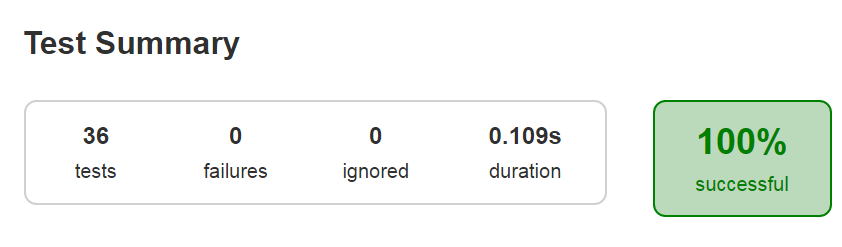
\includegraphics[width=1.0\hsize]{fig/test_summary}
	\caption{Podsumowanie testów}
	\source{Wygenerowane przez Gradle}
\end{figure}

\subsection{Generowanie kodu}
Kod wygenerowany jest OK.

\subsection{NFC i GPS}
Odpowiednie zdarzenia odpalały się w odpowiednich sytuacjach.


\chapter{Korzystanie z frameworku}
Pisanie własnej gry przy użyciu frameworku Adventure Maker jest bardzo proste. Wymaga ono jednak przygotowania środowiska pracy.
W tym rozdziale zawarłem instrukcje dotyczące instalacji, konfiguracji i korzystania z potrzebnych narzędzi. 
\section{Konfiguracja środowika}
Aby móc korzystać z frameworku należy pobrać i zainstalować IDE IntelliJ Idea, JRE, JDK i Android SDK oraz wtyczkę AML.
\subsection{JRE}
JRE, czyli Java Runtime Enviroment, to środowisko uruchomieniowe Javy. Jest ono niezbędne do uruchomienia oprogramowania napisanego napisanego w technologii Java. JRE należy pobrać ze strony producenta [] w wesji 1.8 i zainstalować w standardowy sposób.
\subsection{JDK}
JDK, czyli Java Development Kit, standardowy zestaw narzędzi wykorzystywanych do tworzenia aplikacji w technologii Java. JDK należy pobrać ze strony producenta [] w wesji 1.8 i zainstalować w standardowy sposób.
\subsection{IDE - IntelliJ Idea}
IDE IntelliJ Idea można pobrać ze strony producenta []. Wersja community jest darmowa i wystarczająca do działania frameworku.
Podczas instalacji należy pamiętać o włączeniu pluginu obsługującego aplikacje pisane na system Android.
\subsection{Android SDK}
Android SDK (Standard Development Kit) to standardowy zestaw narzędzi programisty Android pozwalający na tworzenie aplikacji na ten system, w języku JAVA. SDK należy poprać ze strony [] i zainstalować w dowolnej lokalizacji.
\subsection{Wtyczka AML}
Wtyczka AML jest odpowiedzialna za obsługę języka AML, w tym generowanie kodu Java na podstawie pliku ".aml". 

Do prawidłowego działania wtyczki AML potrzebne są wtyczki Xtext i Xtend, które można pobrać ze strony producenta [https://eclipse.org/Xtext/download.html].
Wtyczkę AML należy pobrać [mój link] i zainstalować przyciskiem zainstalować ręcznie.

\section{Przygotowanie projektu}
Przed rozpoczęciem pracy na własnym projektem należy poprać repozytorium []. Znajdujący się w nim projekt ExampleAdventure, jest projektem przykładowej gry. Najłatwiejszym sposobem nie jego wykorzystanie jest skopiowanie go i posługiwanie się nim jako szablonem. Należy pamiętać, aby zmienić id aplikacji w pliku "

\section{Implementacja gry}
Implementacja własnej gry sprowadza się do edycji jednego pliku, mianowicie "game.aml". Należy w nim umieścić kod w języku AML. Kod musi  zawierać wszystkie niezbędne elementy gry. Pisząc ten kod można posłużyć się dokumentacją języka AML zamieszczoną w niniejszej pracy. Warto też wzorować się na kodzie przykładowej gry, który równiej wchodzi w jej skład.

\section{Kompilacja projektu}
Projekt jest standardowym projektem Androidowym, tak więc możemy go też uruchomić przyciskiem play dostępnym w IDE IntelliJ Idea. Ważne jest, żeby korzystać z IDE, nawet w przypadku korzystania z gradle [], ponieważ kod, generowany na podstawie pliku AML, tworzony jest przez samo środowisko.

\chapter{Adventure Maker Language} 
Adventure Maker Language to język domenowy stworzony specjalnie na potrzeby frameworku Adventure Maker. Poniżej znajduje się jego dokumentacja.

\section{Struktura pliku AML} 
Plik AML definiuje wszystkie dostępne w grze elementy. Plik może zawierać dowolną ilość postaci, przedmiotów, lokacji oraz zdarzeń. Dodatkowo należy w nim umieścić warunki początkowe. 

\section{Przygody początkowe} 
Warunki początkowe definiują przygody dostępne od początku gry. Definicja bloku przygód początkowych rozpoczyna się od słów kluczowych
"adventure on start". Następnie w nawiasach klamrowych znajduje się dowolna liczba deklaracji przygód dostępnych na początku gry.
Każda taka definicja składa się z nazwy przygody słówka kluczowego "at" i nazwy lokacji.

Poniższy przykład zawiera definicje składającą się z dwóch przygód "MysteriusMan" i "Bandits", ulokowanych odpowiednio w "OldHouse" i "Forest".
\begin{lstlisting}
adventure on start {
	MysteriusMan at OldHouse
	Bandits at Forest
}
\end{lstlisting}
\section{Klasy Postaci}
Definicja Klasy, inaczej typu postaci to informacje na temat statystyk oraz umiejętności dostępnych dla danej Klasy postaci. Statystyki dzielą się na statystyki początkowe, które postać otrzymuje przy starcie gry, oraz statystyki poziomowe, które zwiększają statystyki postaci z każdym zdobytym poziomem. Umiejętności zostały zorganizowane w postaci drzewa. Aby odblokować daną umiejętność, gracz musi najpierw odblokować wszystkie prowadzące do niej umiejętności.

Definicja typu postaci rozpoczyna się od słów kluczowych "character type". Następnie należy podać nazwę typu za którą znajdują się nawiasy klamrowe. W nawiasach klamrowych należy umieścić kolejno:
\begin{itemize}
	\item statystyki początkowe
	\item statystyki poziomowe
	\item drzewo umiejętności
\end{itemize}

Definicja statystyk początkowych rozpoczyna się od słów kluczowych "stats on start:". Za tymi słowami umieszczone są ilościowe parametry siły, inteligencji i zwinności oznaczone odpowiednio słowami kluczowymi "str", "int", "agi", będącymi skrótami od angielskich tłumaczeń tych parametrów.

Definicja statystyk poziomowych jest bardzo podobna to tych startowych. Występują tu dwie różnice. Po pierwsze, definicja zaczyna się od swój kluczowych "stats per lvl:". Pod drugie przed każdym parametrem występuje znak plusa, który podkreśla fakt, że są to wartości, które zwiększają statystyki postaci. 

Definicja drzewa umiejętności rozpoczyna się od słów kluczowych "skills tree:". Dalej znajduje się dowolna liczba gałęzi drzewa.
Każdy gałąź składa się z nazwy umiejętności, której dotyczy oraz opcjonalnie zbioru gałęzi potomnych, które definiują umiejętności.
Zbiór gałęzi potomnych definiuje się w nawiasach klamrowych poprzedzonych symbolem "=>". 

Poniżej znajduje się przykład definicji postaci typu "Wizard":
\begin{lstlisting}
character type Wizard {
	stats on start:
		10 str
		20 int
		15 agi
	stats per lvl:
		+ 1 str
		+ 2 int
		+ 1 agi
	skills tree:
		Fireball => {
			Wirewall
			BlackMagic
		}
		Poisoning
}
\end{lstlisting}
Z definicji można odczytać, że postać typu "Wizard" otrzymuje 10 punktów siły, 20 inteligencji i 15 zwinności na początku gry.
Otrzymuje też 1 punkt siły, 2 inteligencji i 1 zwinności z każdym zdobytym poziomem doświadczenia.
Na początku może odblokować umiejętność "Fireball" lub "Poisoning". Odblokowanie umiejętności "Fireball" pozwala ponadto na odblokowanie dwóch kolejnych: "Wirewall" i "BlackMagic". 

\section{Typy Przedmioty}
Przedmiot to element, który stanowi nagrodę za pokonanie przeciwnika i może być wykorzystany w celu podniesienia statystyk postaci. 
Definicja przedmiotu jest bardzo prosta. Wystarczy podać jego nazwę, typ oraz wartości premii do odpowiednich statystyk.
Wartości premii umieszczone są w nawiasach klamrowych i składają się z wartości liczbowej poprzedzonej znakiem plus oraz słówka kluczowego "agi", "str" lub "int" odnoszącego się do odpowiedniego typu statystyk. Przedmiot nie musi zawierać bonusu do każdego typu statystyk.

Poniżej znajduje się przykład definiujący przedmiot typu "Sword", zwiększający siłę postaci o 4, a zwinność o 3 punkty.
\begin{lstlisting}
item Sword (weapon) {
	+ 4 str
	+ 3 agi
}
\end{lstlisting}

\section{Definicja Lokacji}
Lokacja to miejsce do którego można się odwołać definiując zdarzenie. Miejsce takie oznacza pewien obszar w fizycznym świecie np. pokój albo kawałek lasu. Lokacje możemy definiować na dwa sposoby za pomocą technologii GPS lub NFC. 
W przypadku technologii GPS lokacje opisuje okrąg o środku wyrażonym jako współrzędne geograficzne i promieniu wyrażonym w metrach. Użycie tej technologii zalecane jest do opisu obszarów znajdujących się na otwartej przestrzeni 
Opisując lokacje za pomocą technologii NFC wystarczy podać odpowiedni tag. Tą technologię należy wykorzystać do opisu przestrzeni zamkniętych jak np. pokoje. Trzeba pamiętać, że odpowiedni znacznik NFC musi znajdować się w tym pomieszczeniu.

Definicja lokacji rozpoczyna się od słowa kluczowego "location" i nazwy. Jeżeli lokacja wyrażona ma być przez znacznik NFC należy użyć słów kluczowych "tagged as", a następnie podać tekst, który stanowi zawartość tagu. W przypadku korzystania z technologii GPS używa się słów kluczowych "in radius of" po którym podaje się odległość w metrach. Następnie po słowach "meters from" należy umieścić szerokość i długość geograficzną.

Poniżej znajdują się przykłady definicji lokacji "OldHouse" i "Forest". Lokacja "OldHouse" oznaczona jest tagiem "OldHouseLocation", natomiast 
"Forest" to obszar o promieniu 100 metrów od punktu o współrzędnych 54°35'45.9"N, 18°14'42.7"E.
\begin{lstlisting}
location OldHouse tagged as OldHouseLocation
location Forest in radius of 100 meters from 54.596077, 18.245200
\end{lstlisting}

\section{Definicja Przeciwnika}

\section{Definicja Przygody}
Przygody są najważniejszym i najbardziej rozbudowanym elementem definicji w języku AML. 
Definicja każdej przygody składa się z słowa kluczowego "adventure", nazwy Przygody, słów "starts from" oraz Zdarzenia początkowego.

Zdarzenie otoczone jest zawsze nawiasami klamrowymi i może zawierać jedną z definicji:
\begin{itemize}
	\item Zdarzenie warunkowe
	\item Pytanie
	\item Walka
	\item Modyfikacja zdarzeń
	\item Blok zdarzeń
	\item Komunikat
\end{itemize}

Zanim pokażę przykładową definicję, omówić z osoba każdy typ Zdarzeń.
\subsection*{Komunikat}
Komunikat to najprostsze ze Zdarzeń. Polega na zwykłym wyświetleniu komunikatu, z którym gracz ma się zapoznać.

Definicja Komunikatu składa się ze słowa kluczowego "Show" oraz treści komunikatu.

Poniżej znajduje się przykład kodu wyświetlającego komunikat "Hello World!".
\begin{lstlisting}
Show "Hello World!"
\end{lstlisting}
\subsection*{Walka}
Walka oznacza zdarzenie polegające na pojedynku z pojedynczym przeciwniku lub ich grupą. Zdarzenie tego typu zawiera informacje o ilości i typu przeciwników, oraz zdarzeniach wywołanych w przypadku zwycięstwa jak i porażki.

Definicja walki rozpoczyna się od słów kluczowych "Fight with". Następnie należy wymienić nazwy wszystkich przeciwników oddzielając je przecinkami. Dalej można umieścić opcjonalnie blok zdarzeń wywołanych w przypadku zwycięstwa oraz blok zdarzeń wywołanych w przypadku porażki.

Definicja bloku zdarzeń wywołanych w przypadku zwycięstwa i porażki rozpoczyna się od słów kluczowych odpowiednio "If win" i "If lost". Dalej znajduje się bloku zdarzeń umieszczonych w nawiasach klamrowych.

Poniżej znajduje się przykładowa definicja bloku walki:
\begin{lstlisting}
Fight with Troll, Orc
If win {
	{Remove VillageInDanger at Forest}
	{Get MagicSword}
}
If lost {
	{Remove VillageInDanger at Forest}
	{Show "Niestety nie udało ci się uchronić mieszkańców wioski"}
}
\end{lstlisting}
Z definicji wynika, że gracz będzie musiał się zmierzyć z dwoma przeciwnikami o nazwach "Troll" i "Orc". Jeżeli ich pokona zdobędzie "MagicSword" w przeciwnym wypadku zostanie wyświetlony komunikat "Niestety nie udało ci się uchronić mieszkańców wioski". W obu przypadkach zdarzenie "VillageInDanger" nie będzie już dłużej dostępne w lokacji "Forest".

\subsection*{Blok Zdarzeń}
Blok Zdarzeń to jedno lub więcej zdarzeń umieszczonych w nawiasach klamrowych.
Poniższy przykład pokazuje blok składający się z 3 zdarzeń.
\begin{lstlisting}
{
	{Remove VillageInDanger at Forest}
	{Get MagicSword}
	{Show "Niestety nie udało ci się uchronić mieszkańców wioski"}
}
\end{lstlisting}

\subsection*{Zdarzenie warunkowe}
Zdarzenie warunkowe służy do zadeklarowania zdarzeń, które wywołane zostaną, tylko w przypadku pewnych warunków. Dodatkowo można zdefiniować zdarzenie alternatywne, wywołane w przypadku niespełnienia warunków.
W aktualnej wersji języka składnia zdarzeń warunkowych jest dość uboga i pozwala jedynie na sprawdzenie, czy postać sterowana przez gracza posiada odpowiednie statystyki.

Definicja zdarzenia warunkowego rozpoczyna się od słów kluczowych "If you have" po których pojawia się wyrażenie warunkowe.
Następnie należy podać definicję zdarzenia. Opcjonalnie można dodać definicje zdarzenia alternatywnego poprzedzając je słowem "else".

Poniżej znajduje się przykład definicji zdarzenia warunkowego: 
\begin{lstlisting}
If you have more str than 30 
{Fight with Orc}
else 
{Show "Walka nie będzie konieczna"}
\end{lstlisting}
Z powyższej definicji wynika, że postać o sile większej niż 30 będzie musiała walczyć z "Orc", natomiast gracz kontrolujący postać słabszą zobaczy komunikat "Walka nie będzie konieczna".

Wyrażenia Warunkowe składają się z słówka kluczowego "more" lub "less", skrótowej nazwy parametru ("str, "agi" lub "int"), słowa "than" oraz wartości liczbowej. Dodatkowo wyrażenia warunkowe można łączyć za pomocą słówek "and" lub "or" oraz nawiasów. Wyrażenie warunkowe można też poprzedzić słowem "no", które wprowadza negacje.

Poniżej znajdują się przykłady wyrażeń warunkowych.

\begin{lstlisting}
If you have no more int than 30
If you have more agi than 20 or more str than 10
\end{lstlisting}
Pierwsze wyrażenie sprawdza, czy postać ma nie więcej niż 30 punktów inteligencji. Drugie sprawdza, czy posiada więcej niż 20 punktów siły lub więcej niż 10 punktów zwinności.

\subsection*{Pytanie}
Pytanie, jest zdarzeniem nieco podobnym do warunkowego, z tą różnicą, że wybór zdarzenia zależy nie od spełnienia, bądź niespełnienia warunków, a od decyzji podjętej przez gracza.

Definicja Pytania zawsze rozpoczyna się od słowa kluczowego "Ask", po którym znajduje się treść wyświetlonego pytania, którą należy podać w cudzysłowie. Po pytaniu należy umieścić jeden lub więcej Odpowiedzi. Odpowiedź składa się ze słowa kluczowego "Answer" oraz "to", pomiędzy którymi należy umieścić treść odpowiedzi (również w cudzysłowie) oraz zdarzenia, do którego prowadzi dana odpowiedź. 

Poniżej znajduje się przykład definicji Pytania:
\begin{lstlisting}
Ask "Chcesz nową zbroję?"
Answer "Tak" to { Get Armor}
Answer "Nie" to { Show "Jak uważasz."}
\end{lstlisting}
Z powyższej definicji wynika, że graczowi zostanie wyświetlone pytanie "Chcesz nową zbroję?". Gdy odpowie "Tak", otrzyma przedmiot o nazwie "Armor". W przeciwnym wypadku ujrzy komunikat "Jak uważasz.".


\subsection*{Modyfikacja Przygód}
Modyfikacja Przygód służy do dodawania lub usuwania przygód z lokacji. 
Definicja zdarzenia dodającego nową Przygodę rozpoczyna się od słowa "Add", a usuwającego "Remove". Następnie należy podać nazwę Przygody i opcjonalnie częstość jej występowania w nawiasach (domyślna częstość wynosi 1). Dalej należy podać lokację, której dotyczy edycja poprzedzając ją słowem "at.

Poniżej znajduje się kilka przykładów Modyfikacji Przygód. 
\begin{lstlisting}
{Add Bandits (4) at Forest}
{Add VillageInDanger at Forest}
{Remove MysteriusMan at OldHouse}
\end{lstlisting}
Pierwsze dwie linie dodają odpowiednio Przygody "Bandits" i "VillageInDanger" do Lokacji las. Przygoda "Bandits" będzie występowała czterokrotnie częściej niż "VillageInDanger". Ostania linia usuwa Przygodę "MysteriusMan" z Lokacji "OldHouse".

\subsection*{Przykład}
Poniżej znajduje się przykład kompletnej definicji przygody.
\begin{lstlisting}
adventure MysteriusManAd starts from {
	Ask "Are you ready to fight?"
	Answer "No" to { Fight with MysteriusManTraining }
	Answer "Yes" to {
		If you have more str than 30 or more int than 30 or more agi than 30 {
			Fight with MysteriusMan
			If win {
				{Show "Great. Now, you are ready for fight with Dragon"}
				{Add BigDragon at Hills}
				{Remove MysteriusManAd at OldHause}
			}
		}
		else {Show "I don't think so"}
	}
}
\end{lstlisting}
Przygoda "MysteriusManAd" rozpoczyna się od pytania "Are you ready to fight?". Odpowiedź "No" prowadzi do walki z "MysteriusManTraining".
Odpowiedź "Yes" prowadzie od efektu zależnego od statystyk postaci. Postać posiadająca przynajmniej jedną ze statystyk na poziomie powyżej 30 punktów, będzie musiała stoczyć Walkę z "MysteriusMan". Jeżeli gracz zwycięży w walce otrzyma komunikat "Great. Now, you are ready for fight with Dragon", odblokuje Przygodę "BigDragon" w lokacji "Hills", a przygoda "MysteriusManAd", nie będzie dłużej dostępna w "OldHause". Postać niespełniająca warunków otrzyma po prostu komunikat "I don't think so". 

\chapter{Przykładowa gra}
Aby ułatwić zrozumienie i korzystanie z frameworku postanowiłem przygotować przykładową grę. Kod AML potrzebny do skompilowania gry znajduje się w załączniku.

\section{Opis scenariusza}

Ponieważ Adventure Maker powstał w ramach pracy dyplomowej postanowiłem, że tematem gry nie będzie oklepane ratowanie księżniczek i walka ze smokami w świecie fantasy, a studiowanie. Okazało się, że pomimo, że framework, nie został zaprojektowany z myślą o grach tego typu, bez problemu udało mi się ją napisać w języku AML.

Akcja gry rozgrywa się na uniwersytecie, a celem gracza jest zdanie egzaminu magisterskiego. Aby to osiągnąć, gracz musi rozwijać umiejętności swojej postaci poprzez zdawanie pomniejszych egzaminów. Kiedy, gracz będzie już gotowy do ostatecznej próby, musi udać się do specjalnej sali, w której może podejść do egzaminu i zdobyć uprawniony dyplom.

Gracz może osiągnąć cel obierając jedną z dwóch strategii. Na początku gry musi podjąć decyzję, czy chcę podążać szlachetną ścieżką dobrego studenta, czy też iść na łatwiznę i oszukiwać. Gra zawiera element moralizatorski, ponieważ wybierając ścieżkę oszusta, można co prawda zdać wszystkie pomniejsze egzaminy, ale ostatecznie gracz i tak skazany jest na porażkę. Gra zaimplementowana jest w taki sposób, żeby podczas egzaminu dyplomowego niewiedza nieuczciwego studenta wyżła na jaw, uniemożliwiając mu tym samym zakończenie studiów.

\section{Uruchamianie gry}

Grę można pobrać [] i zainstalować na dowolnym urządzeniu z systemem android w wersji powyżej 4.0, obsługującym komunikację NFC. Przed rozpoczęciem gry należy zaprogramować i umieścić znaczniki NFC zawierające tagi:
\begin{itemize}
	\item ExamClassRoom
	\item PlainClassRoom
\end{itemize}
Znaczników "PlainClassRoom" można przygotować dowolną ilość i rozmieścić je w kilku salach uczelni. Znacznik "ExamClassRoom" powinien znajdować się w pojedynczej sali, w której odbywać się będą egzaminy dyplomowe.

Po takim przygotowaniu można już swobodnie rozpocząć rozgrywkę.

% załączniki (opcjonalnie):
\appendix
\chapter{Tytuł załącznika jeden}

\begin{lstlisting}

skill BasicKnowledge {
	effect : take (3 * int) damage
	mp : 12
	cooldown : 1 turns
}

skill BrilliantIdea {
	effect : take (4 * int) damage
	mp : 20
	cooldown : 2 turns
}

skill Focusing {
	effect : take (12 * int + 13 * agi) damage
	mp : 60
	cooldown : 4 turns
}

skill AwesomeFocusing {
	effect : take (12 * int + 13 * agi) damage
	mp : 60
	cooldown : 4 turns
}

character type GoodStudent {
	stats on start:
	10 str
	20 int
	10 agi
	stats per lvl:
	+ 1 str
	+ 2 int
	+ 1 agi
	skills tree:
	BasicKnowledge => {
		BrilliantIdea
		Focusing => {AwesomeFocusing}
	}
}

skill PaperCheatsheet {
	effect : take 2*agi damage
	mp : 10
}

skill Smartphone {
	effect : take 2*agi damage
	mp : 10
}

skill FriendHelp {
	effect : take 2*agi damage
	mp : 10
}

skill Luck {
	effect : take 2*agi damage
	mp : 10
}

character type Cheater {
	stats on start:
	10 str
	10 int
	20 agi
	stats per lvl:
	+ 1 str
	+ 1 int
	+ 2 agi
	skills tree:
	Luck => {
		PaperCheatsheet
		FriendHelp
		Smartphone
	}
}

item FunnyHat (helmet) {
}

item GoodPen (weapon) {
	+ 12 str
}

item GoodGrade (armor) {
	+ 12 str
}

item Diploma (armor) {
	+ 10 agi
	+ 10 str
	+ 10 int
}

item WarmGloves (gloves) {
	+ 1 str
}

item BrandNewSmartPhone (weapon) {
	+ 5 int
}

opponent SimpleExam {
	power : 10
	hp : 20
	exp : 100
	loot : GoodGrade 50%, FunnyHat 1 %, BrandNewSmartPhone 10%, GoodPen 20%, WarmGloves 10%
}

opponent MasterDegreeExam{
	power : 50
	hp : 100
	exp : 1000
	loot : Diploma 100%
}

adventure NotAStudent starts from {
	Show "You are not a Student"
}

adventure SimpleExamAdventure starts from {
	Fight with SimpleExam
	If win {
		{
			If you have more int than 30 {
				{Show "You are ready for MasterDegreeExam" }
				{Remove SimpleExamAdventure at ClassRoom}
				{Add MasterExamAdventure at ClassRoom}
			}
			else {
				Show "You have to pass few more exams."
			}
		}
		{
			If you have more agi than 30 {
				{Show "You was catched on cheating." }
				{Add NotAStudent at ClassRoom}
				{Remove SimpleExamAdventure at ClassRoom}
			}
		}
	}
}

adventure MasterExamAdventure starts from {
	{Show "Have you passed all exams?"}
	{
		Fight with MasterDegreeExam
		If win {
			{Show "Great. You just have gradueted your Master Degree"}
			{Remove MasterExamAdventure at MasterExamRoom}
		}
		If lost {
			Show "You can try another one"
		}
	}
}

location ClassRoom tagged as ClassRoom
location MasterExamRoom tagged as MasterExamRoom

adventure on start {
	SimpleExamAdventure at ClassRoom
}

\end{lstlisting}

% literatura (obowiązkowo):
\bibliographystyle{unsrt}
\bibliography{xml}

% spis tabel (jeżeli jest potrzebny):
\listoftables

% spis rysunków (jeżeli jest potrzebny):
\listoffigures

\oswiadczenie

\end{document}
